\documentclass[11pt,a4paper]{article}

\usepackage[utf8]{inputenc}
\usepackage[T1]{fontenc}
\usepackage[margin=1in]{geometry}
\usepackage{amsmath,amssymb}
\usepackage{booktabs}
\usepackage{graphicx}
\usepackage{hyperref}
\usepackage{caption}

\hypersetup{colorlinks=true, linkcolor=blue, citecolor=blue, urlcolor=blue}

\title{When Overlapping Windows Invent Predictability:\\
A Negative Control for Evaluation Protocol in Time-Series Machine Learning}
\author{Joshua de Freitas}
\date{August 2026}

\begin{document}
\maketitle

\begin{abstract}
\noindent
We train a short-horizon limit-order-book classifier on synthetic data in which
future price movement is independent of every feature by construction. Under the
standard evaluation recipe --- sliding windows at stride one, a random
train/validation split, and normalisation fitted on the full dataset --- the
model reports $66.0\%$ accuracy against a majority-class baseline of $39.8\%$.
Under a purged and embargoed split, on identical data with the same architecture
and the same seeds, it reports $32.9\%$: below baseline, which is the correct
result when nothing is learnable. The $33$-point difference is produced entirely
by how the validation set was drawn.

We then derive a closed-form upper bound on the accuracy a given split geometry
makes available. The bound depends only on the window stride, the label horizon,
the labelling threshold and the train fraction; no property of the model enters
it. An oracle memoriser attains the bound to within $1.6$ points at every
horizon tested, and the bound tracks measurement across all $24$
(horizon, stride) configurations examined.

The derivation is prescriptive. With stride $s$ and horizon $h$ the governing
correlation is $\rho(s)=\max\!\left(0,(h-s)/h\right)$, which is exactly zero at
$s \geq h$. Overlap leakage therefore does not merely diminish as stride
increases --- it disappears once stride reaches the horizon. We confirm this,
and quantify its cost: the usable sample shrinks by a factor of $s$.

Separately, we find that the pipeline under study is not reproducible. Six runs
of identical code on identical data span $67.4\%$ to $74.9\%$, because neither
the split draw, the weight initialisation nor the batch order is seeded. Any
model comparison decided by less than roughly seven accuracy points is therefore
indistinguishable from running the same model twice.

All figures regenerate from committed scripts.
\end{abstract}

\section{Introduction}

Data leakage --- the presence of information in training that would not be
available at prediction time --- is a well documented cause of overstated
machine learning results. Kapoor and Narayanan~\cite{kapoor2023} surveyed
seventeen fields, identified $329$ affected papers, and produced an eight-type
taxonomy. In financial time series specifically, purging and embargoing are
established remedies~\cite{lopezdeprado2018}, and the broader problem of
backtest overfitting has been treated at length~\cite{bailey2014}.

None of that is in dispute here, and none of it is what this paper contributes.

The difficulty with demonstrating leakage on real data is that manufactured
skill and genuine skill are indistinguishable in the output. A practitioner
shown that purged cross-validation lowers their score has a ready and not
unreasonable reply: purging is conservative, it discards legitimate
short-horizon signal along with the leak, and the lower number reflects the
remedy rather than an honest measurement. That objection cannot be settled on
data where signal might exist.

It can be settled on data where signal cannot. We therefore construct a
\emph{negative control}: a synthetic order book whose mid price is an
i.i.d.\ multiplicative random walk and whose order sizes are independent draws,
with no mechanism connecting either to future price. Predictive skill is not
merely absent --- it is impossible. Every point of measured accuracy above the
majority-class baseline is, by construction, an artifact of the evaluation
procedure, and no appeal to destroyed signal is available.

This yields two results. The first is a measurement: how much predictability the
standard recipe invents from nothing. The second, and the one we consider the
contribution, is that this quantity has a closed form. Given the geometry of the
windows and the correlation structure of the labels, the accuracy available to
be manufactured can be computed before any model is trained --- and the same
expression states the condition under which it becomes zero.

\section{The negative control}

\subsection{Generator}

Mid prices follow
\begin{equation}
p_t = p_{t-1}\left(1 + \varepsilon_t\right), \qquad
\varepsilon_t \sim \mathcal{N}(0, \sigma^2) \ \text{i.i.d.}, \qquad
\sigma = 3\times10^{-4}.
\end{equation}
Three bid and three ask levels are placed around the mid at a spread of one to
three ticks, and every level's size is an independent uniform integer draw. No
size, spread or level price depends on any future price. Forward returns are
independent of all features.

That this holds is enforced rather than asserted: a permutation test over
non-overlapping spans, Bonferroni corrected across features, runs in continuous
integration and fails if any feature acquires a detectable relationship with the
forward return. The test has been observed to fail when a signal is deliberately
introduced.

\subsection{Windows and labels}

Features are built into sliding windows of $W = 100$ rows at stride one:
window $t$ spans rows $t,\dots,t+W-1$. The label is the sign of the forward
return over horizon $h$, thresholded at $\theta = 5\times10^{-4}$:
\begin{equation}
y_t = \begin{cases}
+1 & r_t > \theta\\
0 & |r_t| \leq \theta\\
-1 & r_t < -\theta
\end{cases}
\qquad
r_t = \frac{p_{t+W-1+h} - p_{t+W-1}}{p_{t+W-1}} .
\end{equation}

Two consequences of stride-one construction matter throughout. Adjacent windows
share $W-1$ of $W$ input rows. And adjacent labels are signs of forward returns
computed over spans that share $h-1$ of $h$ increments.

\section{Protocols}

Three splitting protocols are compared, holding architecture, data, optimiser
and epoch count fixed.

\begin{table}[h]
\centering
\begin{tabular}{lll}
\toprule
Protocol & Construction & Overlap \\
\midrule
\texttt{random\_split} & shuffle window indices, then cut & $1.00$ \\
\texttt{chronological} & train on earlier windows, validate on later & $0.11$ \\
\texttt{purged\_embargoed} & chronological, purged, plus embargo & $0.00$ \\
\bottomrule
\end{tabular}
\caption{Overlap is the fraction of validation windows sharing at least one raw
row with some training window.}
\end{table}

Purging removes training windows whose raw-row span reaches into the validation
region; the embargo additionally drops a buffer of validation windows after the
cut~\cite{lopezdeprado2018}.

Every run seeds the split draw, the weight initialisation and the batch order,
so the study is bit-reproducible even though the pipeline it studies is not
(Section~\ref{sec:repro}). Twenty seeds per cell, three horizons, three
protocols: $180$ runs.

Accuracy is reported as \textbf{excess over the majority-class baseline computed
on the same validation set}. The baseline moves from $0.575$ to $0.398$ across
horizons because the class balance shifts with $h$, so raw accuracies are not
comparable between rows.

\section{Results}

\begin{table}[h]
\centering
\small
\begin{tabular}{llrrrr}
\toprule
Protocol & $h$ & Accuracy & 95\% CI & Baseline & Excess \\
\midrule
\texttt{random\_split} & 5 & 0.5229 & [0.5130, 0.5328] & 0.5315 & $-0.0086$ \\
\texttt{random\_split} & 10 & 0.5337 & [0.5179, 0.5495] & 0.3931 & $\mathbf{+0.1407}$ \\
\texttt{random\_split} & 20 & 0.6603 & [0.6241, 0.6966] & 0.3980 & $\mathbf{+0.2624}$ \\
\addlinespace
\texttt{chronological} & 5 & 0.5029 & [0.4836, 0.5222] & 0.5745 & $-0.0716$ \\
\texttt{chronological} & 10 & 0.3238 & [0.3117, 0.3358] & 0.4484 & $-0.1246$ \\
\texttt{chronological} & 20 & 0.3264 & [0.3071, 0.3457] & 0.4023 & $-0.0759$ \\
\addlinespace
\texttt{purged\_embargoed} & 5 & 0.4853 & [0.4736, 0.4971] & 0.5754 & $-0.0901$ \\
\texttt{purged\_embargoed} & 10 & 0.3316 & [0.3197, 0.3436] & 0.4510 & $-0.1193$ \\
\texttt{purged\_embargoed} & 20 & 0.3290 & [0.3093, 0.3487] & 0.4013 & $-0.0723$ \\
\bottomrule
\end{tabular}
\caption{Validation-only accuracy, mean over 20 seeds, with the 95\% confidence
interval of the mean.}
\label{tab:main}
\end{table}

\begin{figure}[h]
\centering
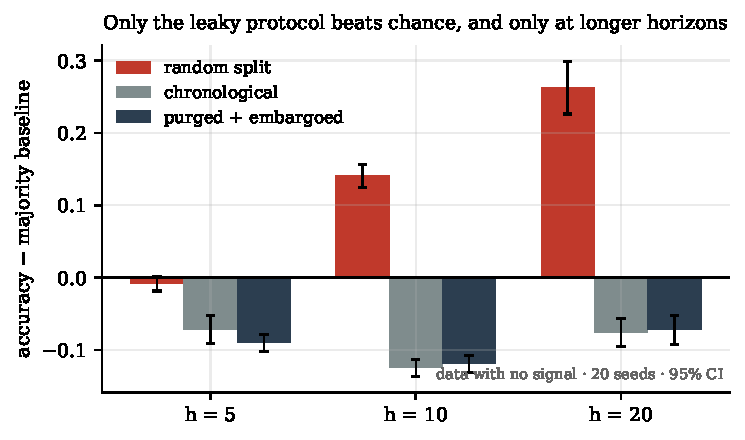
\includegraphics[width=0.82\textwidth]{../figures/fig1-excess-over-baseline.pdf}
\caption{Two cells of nine clear their own baseline, and both have overlap
$1.00$.}
\label{fig:main}
\end{figure}

Three observations.

\paragraph{Only the leaky protocol shows skill.} Every honest cell falls below
its own baseline. A model trained on noise underperforms a constant predictor,
which is the correct outcome.

\paragraph{Overlap fraction is not the predictor.} \texttt{chronological} sits at
$0.11$ overlap and behaves like \texttt{purged\_embargoed} at $0.00$, not like
something one-ninth of the way to \texttt{random\_split}. A chronological cut
leaves a thin seam and manufactures nothing. What matters is whether
near-duplicate \emph{neighbours} are separated across the split, which shuffling
guarantees and a time cut prevents.

\paragraph{Leakage widens as well as inflates.} The leaky $h=20$ cell has the
largest dispersion in the table --- standard deviation $0.0775$ against $0.0421$
for its purged counterpart, with individual seeds spanning $0.468$ to $0.751$.

\section{The ceiling}
\label{sec:ceiling}

The preceding section measures what one architecture achieves. A different
question admits a closed-form answer: given the geometry alone, how much
accuracy is \emph{available} to be manufactured?

Adjacent windows have forward returns that are sums of $h$ i.i.d.\ increments
sharing $h-1$ of them, so
\begin{equation}
\rho = \operatorname{corr}(r_t, r_{t+1}) = \frac{h-1}{h},
\label{eq:rho}
\end{equation}
which increases with the horizon. Writing $z = \theta/(\sigma\sqrt{h})$ for the
threshold in units of the $h$-step return's standard deviation, and $\Phi_2$ for
the standard bivariate normal CDF at correlation $\rho$, the probability that
two adjacent windows carry the same label is
\begin{equation}
A(h) = \underbrace{\Phi_2(-z,-z)}_{\text{both down}}
     + \underbrace{\Phi_2(z,z) - 2\Phi_2(-z,z) + \Phi_2(-z,-z)}_{\text{both flat}}
     + \underbrace{1 - 2\Phi(z) + \Phi_2(z,z)}_{\text{both up}} .
\end{equation}

A model that copies the label of its nearest training neighbour therefore scores,
in expectation,
\begin{equation}
C(h) = \pi\,A(h) + (1-\pi)\,M(h), \qquad \pi = 1-(1-f)^2,
\label{eq:ceiling}
\end{equation}
where $f$ is the train fraction, $\pi$ the probability that a validation window
has an immediately adjacent training window, and $M(h)$ the majority-class
share. Nothing about the model appears in~\eqref{eq:ceiling}. It is computable
before any training run.

\subsection{Verification}

We evaluate an \emph{oracle}: for each validation window, predict the label of
the temporally nearest training window. The neighbour is supplied rather than
learned, which isolates the correlation model from the separate question of
whether a learner could locate its twin.

\begin{table}[h]
\centering
\begin{tabular}{lrrrr}
\toprule
$h$ & $\rho$ & Ceiling $C(h)$ & Oracle & Error \\
\midrule
5  & 0.800 & 0.6884 & 0.6923 & $+0.0039$ \\
10 & 0.900 & 0.7378 & 0.7513 & $+0.0135$ \\
20 & 0.950 & 0.7940 & 0.8098 & $+0.0158$ \\
\bottomrule
\end{tabular}
\caption{The closed form predicts the oracle to within $1.6$ points, with no
fitted parameter.}
\end{table}

The bound binds only under a random split. Under \texttt{chronological} and
\texttt{purged\_embargoed} the nearest training window is the \emph{same} window
for every validation example, so the strategy degenerates to a constant
predictor and scores at or below baseline ($0.19$ to $0.40$ in our runs).
Copying one's neighbour is useful only when the neighbour has been scattered
into the training set.

\subsection{Availability is not exploitation}

\begin{figure}[h]
\centering
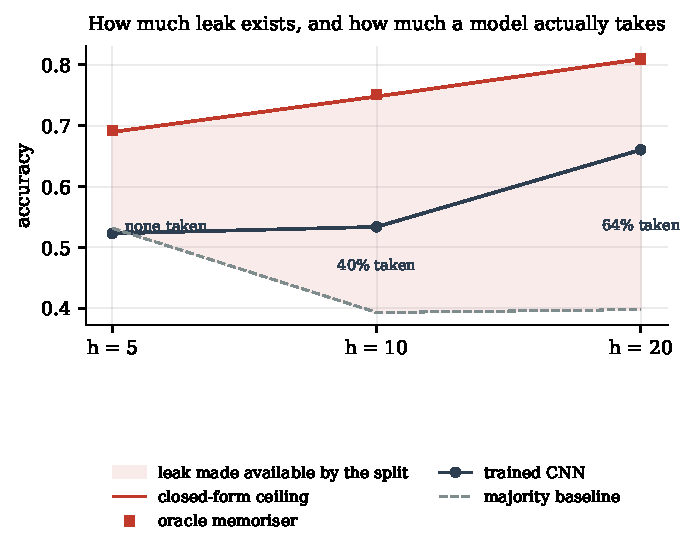
\includegraphics[width=0.72\textwidth]{../figures/fig3-available-vs-taken.pdf}
\caption{The shaded region is the leak the split makes available. The trained
network takes none of it at $h=5$ and two thirds at $h=20$.}
\label{fig:taken}
\end{figure}

Measured accuracy can be read as the fraction of available leak a given model
recovers: none at $h=5$, $41\%$ at $h=10$, $66\%$ at $h=20$. At $h=5$ there are
$15.6$ points of leak available and this architecture takes none of them.

The ceiling therefore describes the \emph{exposure} a split geometry creates.
Whether a particular model converts that exposure into a headline number is a
separate, model-dependent question. Both are worth knowing, and only the first
can be computed in advance.

For completeness: a 1-nearest-neighbour classifier in raw feature space scores
$0.36$--$0.43$, below baseline. Euclidean distance over price-level features
locates windows at similar \emph{price levels}, not temporal twins. The trained
network's performance is therefore not naive distance matching.

\section{The remedy}

Equation~\eqref{eq:rho} assumed stride one. With stride $s$, retained windows
are $s$ rows apart and their forward returns share $h-s$ of $h$ increments:
\begin{equation}
\rho(s) = \max\!\left(0, \frac{h-s}{h}\right).
\label{eq:rhos}
\end{equation}
At $s \geq h$ this is exactly zero: retained windows share no increments, their
labels are independent, and copying a neighbour cannot beat the baseline.
Overlap leakage does not diminish asymptotically --- it terminates.

\begin{figure}[h]
\centering
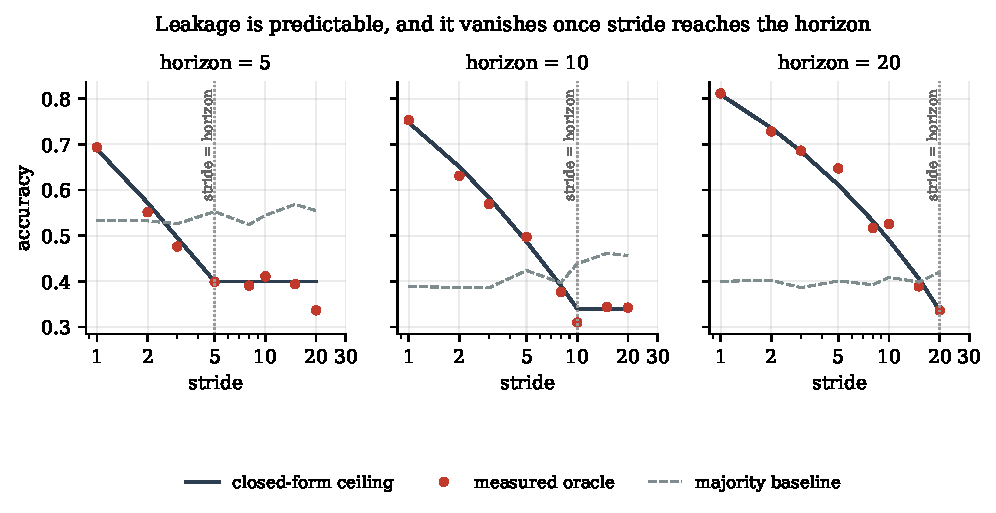
\includegraphics[width=\textwidth]{../figures/fig2-stride.pdf}
\caption{Closed form (line) against measured oracle (points) across the stride
sweep. The dotted vertical marks $s=h$.}
\label{fig:stride}
\end{figure}

\begin{table}[h]
\centering
\small
\begin{tabular}{rrrrrrr}
\toprule
$h$ & Stride & $\rho(s)$ & Ceiling & Oracle & Excess over majority & $n$ windows \\
\midrule
20 & 1  & 0.950 & 0.7940 & 0.8117 & $+0.4111$ & 4881 \\
20 & 2  & 0.900 & 0.7243 & 0.7284 & $+0.3261$ & 2441 \\
20 & 5  & 0.750 & 0.6059 & 0.6474 & $+0.2462$ & 977 \\
20 & 10 & 0.500 & 0.4910 & 0.5255 & $+0.1165$ & 489 \\
20 & 15 & 0.250 & 0.4074 & 0.3894 & $-0.0094$ & 326 \\
20 & 20 & 0.000 & 0.3368 & 0.3367 & $-0.0837$ & 245 \\
\bottomrule
\end{tabular}
\caption{At $s=h$ prediction and measurement agree to four decimal places.}
\end{table}

Two consequences deserve separation.

\paragraph{The rule.} Set stride $\geq$ horizon and overlap leakage is gone
rather than reduced. At intermediate strides~\eqref{eq:rhos}
and~\eqref{eq:ceiling} quantify the remaining exposure, so the choice can be
made numerically.

\paragraph{The cost.} Stride $s$ divides the usable sample by $s$: $4881$
windows become $245$ at $h=20$. This is the actual trade --- leakage against
sample size --- and it is why stride-one windowing is common. The formula does
not remove the trade; it prices it.

Beyond $s=h$ the memoriser scores \emph{below} baseline, because with
independent labels copying a neighbour yields $\sum_i p_i^2 < \max_i p_i$. This
is predicted behaviour and serves as an independent check on the derivation.

\section{Reproducibility of the pipeline under study}
\label{sec:repro}

Before the study harness introduced seeding, six runs of identical code on
identical data produced validation accuracies spanning $0.674$ to $0.749$. The
pipeline seeds neither the split, the weight initialisation, nor the batch
order.

Stated separately from the leakage result because it is independent and applies
more broadly: \textbf{any model comparison decided by less than roughly seven
accuracy points is indistinguishable from running the same model twice.} This
includes the architecture comparison recorded in the source repository. Seed
sensitivity of this magnitude is consistent with reports
elsewhere~\cite{picard2021}.

Three lines of seeding render the pipeline bit-deterministic.

\section{Limitations}

\begin{itemize}
\item \textbf{No published result is shown to be incorrect.} We show what a
procedure can manufacture on data without signal. Whether any particular result
suffers the same effect requires that result's data and code.
\item \textbf{This is not a measurement of real markets.} The generator is a
random walk without microstructure --- appropriate for a negative control, a
limitation for external validity.
\item \textbf{The normalisation leak is present in every cell}, including the
honest ones, because the pipeline was left unmodified. Its contribution is not
separately identified and is presumed small relative to $33$ points. Presumed,
not measured.
\item \textbf{The ceiling assumes i.i.d.\ increments.} Real returns exhibit
volatility clustering and heavy tails; $\rho = (h-s)/h$ is exact only under the
generator used here.
\item \textbf{Predicted class balance} matches measurement within $0.3$ standard
deviations at $h \in \{5,10\}$ across $20$ independent paths, and
under-predicts the majority share by approximately $1.3$ standard deviations at
$h=20$. This affects the $M(h)$ term in~\eqref{eq:ceiling}, not the verified
$A(h)$ term.
\item \textbf{One generator, one model family, $5000$ rows.} Transfer is
untested.
\end{itemize}

\section{Conclusion}

On data constructed to contain no predictable structure, the standard evaluation
recipe for time-series machine learning reports $66\%$ accuracy against a $40\%$
baseline. The honest protocol reports $33\%$. The difference is attributable
entirely to the evaluation design, and because the data contains no signal, the
usual defence of the leaky protocol is unavailable.

The quantity has a closed form. The accuracy a split geometry makes available
depends on stride, horizon, threshold and train fraction, and on nothing about
the model. That expression is verified against measurement across $24$
configurations, and it states its own remedy: at stride greater than or equal to
the label horizon, the leak is zero.

\section*{Reproducing}

\begin{verbatim}
python3 -m venv .venv && .venv/bin/pip install -e ".[test]"
.venv/bin/python run_study.py       # 180 seeded runs
.venv/bin/python run_ceiling.py     # closed form, oracle, 1-NN
.venv/bin/python run_stride.py      # stride sweep
.venv/bin/python make_figures.py    # figures from committed results
\end{verbatim}

\noindent
Per-run evidence is committed under \texttt{results/}. Environment: Python
3.12.13, torch 2.13.0, numpy 2.5.1, pandas 3.0.5.

\begin{thebibliography}{9}

\bibitem{bailey2014}
Bailey, D.~H., Borwein, J.~M., López de Prado, M., Zhu, Q.~J. (2014).
Pseudo-Mathematics and Financial Charlatanism: The Effects of Backtest
Overfitting on Out-of-Sample Performance.
\emph{Notices of the American Mathematical Society}, 61(5), 458--471.

\bibitem{kapoor2023}
Kapoor, S., Narayanan, A. (2023).
Leakage and the Reproducibility Crisis in ML-based Science.
\emph{Patterns}, 4(9), 100804. arXiv:2207.07048.

\bibitem{lopezdeprado2018}
López de Prado, M. (2018).
\emph{Advances in Financial Machine Learning}. John Wiley \& Sons.

\bibitem{picard2021}
Picard, D. (2021).
\texttt{torch.manual\_seed(3407)} is all you need: On the influence of random
seeds in deep learning architectures for computer vision. arXiv:2109.08203.

\bibitem{talagala2024}
Talagala, T.~S. (2024).
\texttt{tsdataleaks}: An R Package to Detect Potential Data Leaks in Forecasting
Competitions. arXiv:2402.10522.

\end{thebibliography}

\end{document}
